% INTRODUÇÃO-------------------------------------------------------------------

\chapter{INTRODUÇÃO}
\label{chap:introducao}

% Importância de estudar o CNV
A variação no número de cópias (\textit{Copy Number Variation}/CNVs) é um dos fatores que contribui para a expansão e diversidade da família de genes, ela foi observada como alterações ocorridas em larga escada de inserções, deleções e duplicações na região genômica \cite{Perry2009,Zhao2013,Redon2006,Costain2016}. 
As CNVs podem ser identificadas como uma variação neutra ou como modificadores de sucessibilidade a doenças \cite{Costain2016,Perry2009}.

% Estratégia de identificar CNV e ligação a doenças
A análise da região genômica pode ser realizada graças as tecnologias desenvolvidas para seu o sequenciamento, permitindo a observação de variantes de DNA \cite{Sathirapongsasuti2011}.
Embora o sequenciamento completo do genoma (\textit{Whole Genome Sequencing}/WGS) seja uma das abordagens utilizada para a investigação de CNVs, o sequenciamento completo do exoma (\textit{Whole Exome Sequencing}/WES) vem se destacando como uma estratégia mais viável, econômica e eficiente no tempo. A viabilidade e eficiência do WES considera que 85\% dos variantes conhecidos ligados a doenças mendelianas encontra-se na área sequenciada \cite{Chong2015,Sathirapongsasuti2011,Fromer2012}.

% Ligação aos modelos estatísticos 
Devido à quantidade, complexidade e ruído dos dados obtidos a partir sequenciamento das regiões codificantes do genoma (exoma), muitas ferramentas de detecção de CNVs foram desenvolvidos para determinar os tipos, as quantidades e as localizações de variações \cite{Fromer2012,Tan2014}. Esses fatores podem ser alcançados com a utilização de modelos estatísticos na descoberta de variações no mapa de dados gerados no WES, essa é uma das abordagens que obteve mais sucesso na integração das ferramentas com o sequenciamento, demonstrando eficiência ao realizar detecções \cite{Tan2014}.

A utilização de modelos estatísticos aplicados para detecção de \textit{copy number variation} visa encontrar pontos de mudanças em uma representação gráfica dos seus dados, assim facilitando a determinação de uma variação de acordo com a localização do ponto de mudança \cite{Zhao2013}. Essa técnica se tornou popular, sendo desenvolvidos diversas ferramentas com o propósito de detectar pontos de mudanças (Change Point Detection/CPD) focadas na análise de CNVs \cite{Olshen2004,Baldi2001,Girimurugan2018,Picard2011,Plagnol2012,Muggeo2010}.

Apesar das diversas técnicas e ferramentas existentes de CPD, nenhuma delas pode identificar todas as CNVs presentes no exoma \cite{Zhao2013}, entretanto, a sua utilização em determinadas situações demonstra resultados diferentes, de acordo com a adaptabilidade do método aos dados, fazendo com que apresentem uma maior efetividade ao encontrar variações. A diferença entre métodos e resultados obtidos pode ser vista ao comparar a execução de cinco algoritmos específicos de detecção de variações no número de cópias na \autoref{fig:ferramentas-cnv} \cite{Muggeo2010}.

\begin{figure}[!htb] 
\centering 
\caption{Segmentação da linha celular de câncer de mama MDA157, onde cada linha representa um cromossomo, indexado ao lado esquerdo} 
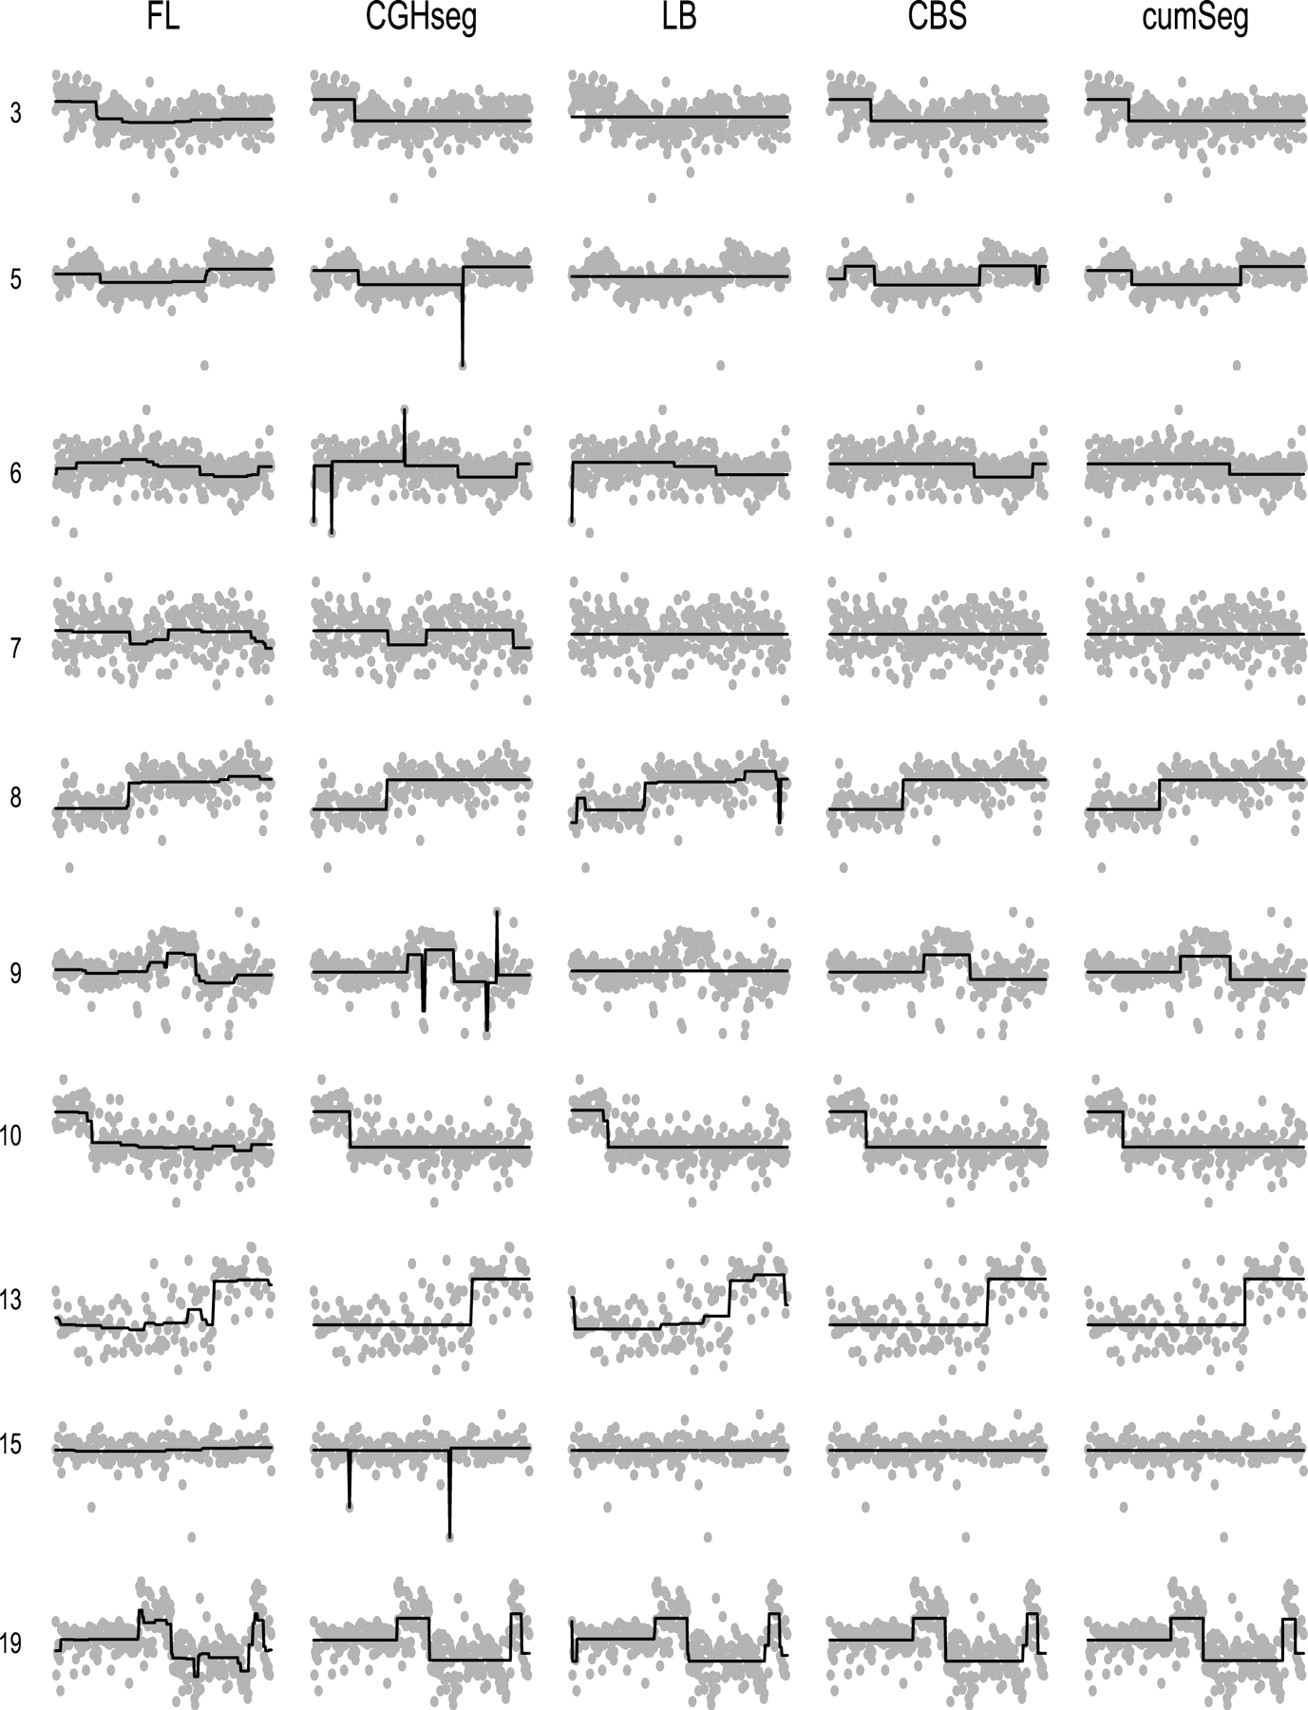
\includegraphics[width=0.8\textwidth]{./dados/figuras/ferramentas-cnv} 
\fonte{\cite{Muggeo2010}} 
\label{fig:ferramentas-cnv} 
\end{figure} 

A \autoref{fig:ferramentas-cnv} demostra que a variação da localização de \textit{change points} relativos a um conjunto de dados (\textit{dataset}), pode apresentar mudanças de acordo com o algoritmo e a técnica implementada para análise na ferramenta. Esse mesmo efeito, também pode ser identificado em comparação de algoritmos de CPD \cite{Ducre-Robitaille2003,Reeves2007}.

O desenvolvimento de técnicas de análises de CPD e CNVs, são frequentes na área da computação, sendo criados diversas teorias e bibliotecas acerca dos assuntos, nos últimos anos \cite{Girimurugan2018,Uzai2019,Chu2019}. A evolução nesse contexto, pode ser observada sobre o viés da busca de melhoria contínua, em relação aos métodos existentes.

Entretanto, apesar de ser realizado testes de validação e comparações com algoritmos semelhantes, por um autor de um método em sua publicação \cite{Uzai2019,Baldi2001}, ainda restam dúvidas sobre a adaptação do mesmo em cenários específicos, ao comparar com ferramentas amplamente difundidas. Portanto, esse trabalho busca reunir dados, estudos e funcionalidades de diferentes ferramentas de CPD em um único ambiente, de modo a especializa-los em leitura de \textit{datasets} de WES na identificação de variações nos números de cópias.

\section{JUSTIFICATIVA}

A necessidade de analisar variações no número de cópias é essencial para a determinação da estrutura do genoma humano e as possíveis modificações sofridas no material genético, já que é a partir dele que as características genéticas são extraídas. O problema de observação e anotação de CNVs é um desafio de pesquisa constante, pois, em alguns casos ela pode ser associada a uma doença, seja ela conhecida ou não \cite{McCarroll2007}. A detecção de variações utilizando pontos de mudanças é uma das abordagens existentes que apresentaram resultados satisfatórios nas análises realizadas, ao adaptar de algoritmos genéricos de CPD com a leitura de dados do exoma \cite{Olshen2004,Picard2011,Girimurugan2018}.

Pensando nisso, a proposta para essa pesquisa é fornecer a disponibilização de métodos existentes de detecção de pontos de mudanças no cenário de dados segmentados do exoma em um único ambiente, buscando identificar a aceitabilidade e eficiência de sua aplicação no contexto proposto. O desenvolvimento dessa pesquisa beneficiará pesquisadores, biólogos, especialistas em genética e pessoas que possuem interesses relacionados ao estudo dos genes e de suas doenças, no que diz respeito da facilidade de execução de diferentes métodos de pontos de mudanças para detecção de CNVs a partir de um único meio.

\section{OBJETIVOS}

\subsection{Objetivo Geral}

Aplicar o conceito de detecção de pontos de mudanças, utilizando diferentes abordagens técnicas desenvolvidas para segmentação de dados de uma série temporal, no contexto de anotação de variações nos números de cópias em uma coleção de dados gerados a partir do WES. O proposito é a obtenção de um ambiente integrado com diversos algoritmos de identificação de ponto de mudança em \textit{datasets} de exoma.

\subsection{Objetivos Específicos}
	
\begin{itemize}
    \item Explicar a importância de \textit{copy number variation}.
    \item Descrever o conceito de \textit{change point detection}, caracterizando com exemplos, os algoritmos desenvolvidos para esse objetivo.
    \item Analisar a aplicabilidade dos algoritmos de CPD para a CNV, citando exemplos dos mesmos.
    \item Desenvolver um ambiente que dispõe de integrações com algoritmos de CPD.
    \item Fornecer um algoritmo focado em leitura de dados de sequenciamento de DNA.
\end{itemize}

\section{ORGANIZAÇÃO DO TEXTO}

Este trabalho se organiza da seguinte forma:

\autoref{chap:introducao} - Introdução: Situa o leitor na área de pesquisa em que o trabalho é focado, definindo o porquê do seu desenvolvimento, os objetivos a serem alcançados com a conclusão e a organização do projeto.

\autoref{chap:fundamentacaoTeorica} - Revisão de Literatura: Apresenta uma pesquisa que contém conceitos e reflexões acerca dos principais temas referentes ao trabalho proposto. Neste capítulo é apresentado a definição de exoma e a importância da sua utilização na descoberta de doenças (\autoref{sec:exoma}), o estudo acerca do surgimento e a evolução de tecnologias capazes de obter os componentes do genoma (\autoref{sec:sequenciamentoDoDna}), a conceituação de CNVs, ressaltando a relevância de sua pesquisa e o uso dos métodos e ferramentas de detecção nessa variação genética (\autoref{sec:copyNumberVariation}), a formulação conceitual de uma das estratégias existentes de análise de CNV, sendo ela o \textit{change point detection}, descrevendo alguns algoritmos desenvolvidos (\autoref{sec:changePointDetection}) e a conceituação de matriz de confusão e suas fórmulas \autoref{sec:matrizDeConfusao}.

\autoref{chap:metodologia} - Metodologia: Discorre sobre os meios e procedimentos adotados, exemplificando e definindo a forma de desenvolvimento e funcionamento de fluxo da ferramenta a ser desenvolvida.

\autoref{chap:planoDeTrabalho} - Plano de Trabalho: Expõe o cronograma adotado para o desenvolvimento do projeto, disponibilizando o início e fim de um conjunto de atividades e sua descrição.

% \autoref{chap:consideracoesFinais} - Considerações Finais: Apresenta as considerações finais acerca do trabalho desenvolvido.